\documentclass{ximera}
 
%% You can put user macros here
%% However, you cannot make new environments

\listfiles

\graphicspath{{./}{firstExample/}{secondExample/}}

\usepackage{tikz}
\usepackage{tkz-euclide}
\usepackage{tikz-3dplot}
\usepackage{tikz-cd}
\usetikzlibrary{shapes.geometric}
\usetikzlibrary{arrows}
\usetikzlibrary{decorations.pathmorphing,patterns}
\usetkzobj{all}
\pgfplotsset{compat=1.13} % prevents compile error.

\renewcommand{\vec}[1]{\mathbf{#1}}
\newcommand{\RR}{\mathbb{R}}
\newcommand{\dfn}{\textit}
\newcommand{\dotp}{\cdot}
\newcommand{\id}{\text{id}}
\newcommand\norm[1]{\left\lVert#1\right\rVert}
 
\newtheorem{general}{Generalization}
\newtheorem{initprob}{Exploration Problem}

\tikzstyle geometryDiagrams=[ultra thick,color=blue!50!black]

\usepackage{mathtools}
 
\title{The Simple Pendulum}
 
\begin{document}
 
\begin{abstract}
An experiment involving a simple pendulum.
\end{abstract}
 
\maketitle
 
 \section*{The Simple Pendulum}
 The purpose of this exercise is to enhance your understanding of linear second order homogeneous differential equations through a modeling application involving a Simple Pendulum which is simply a mass swinging back and forth on a string.  Like the mass on a spring application, this model problem is representative of a wide variety of problems described by second order linear differential equations.  Instructions for constructing and modeling a remarkably simple physical apparatus will guide students in applying the concepts first introduced in Chapter 5 of Trench’s text.
 
 \subsection*{The Experiment}
 A simple pendulum apparatus will be modeled in this experiment.  The following discussion outlines the physical setup.  Later, the mathematical model of the motion is developed.
To try this exercise at home or school, you will need around one meter of string, any small dense object that can be tied to the end of the string, and a measuring tape or ruler.  Optionally, a video camera – such as with a cell phone – can be used to help record your experiment for careful analysis later.  Measurement of amplitude may be easiest if the object is hung in front of a marked wall or blackboard or above a surface where the measuring tape is visible.  If a chalkboard or whiteboard is not available, you could tape paper to a surface and mark distances as desired to help visualize the swinging.
In the following example, a combination lock is hung from 1 meter of string in front of a blackboard.  The string is attached to a post that sticks out a few inches from the blackboard so that the lock does not come in contact with the board.  To make it easier to monitor the amplitude of the motion, marks are made every two centimeters.  The lock will be released at the $20$ centimeter position, with a corresponding angle that is small enough that the following mathematical model will give good predictions.

\begin{image}
 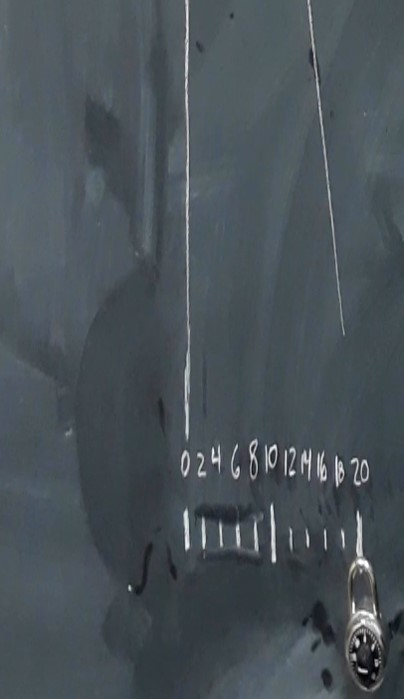
\includegraphics[height=1.5in]{pendulumLock.jpg}
\end{image}

\subsection*{The Simple Pendulum Model from a Mathematical Perspective}

Trench reviews an undamped pendulum in Example 4.4.2 (in section 4.4).  A weight of mass m is attached to the end of a weightless rod (or string) of length L that rotates on a frictionless axle.  The mass could move in a large circular arc:

\begin{image}
 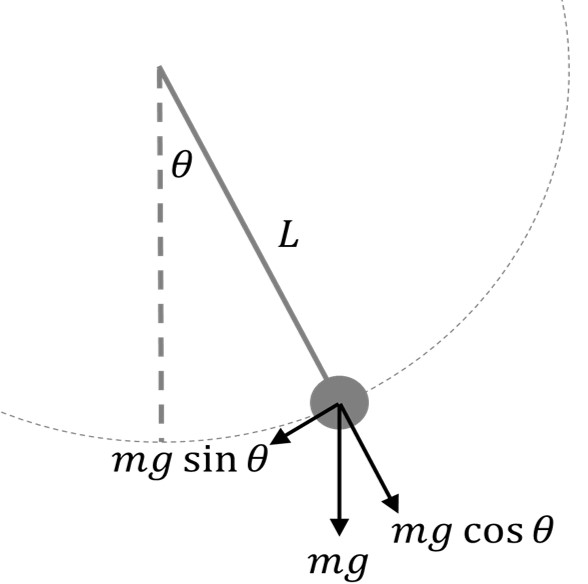
\includegraphics[height=1.5in]{pendulumswing.jpg}
\end{image}

To begin, we will neglect air resistance.  Newton’s second law of motion stipulates that the product of m and the tangential acceleration $L\theta''$ will be equal to the tangential component of the gravitational force:
$$mL\theta''=-mg \sin\theta $$
Cancelling mass on each side and writing in standard form gives:
$$\theta ''+\frac{g}{L} \sin\theta=0$$
When the angle θ is small, perhaps less than 15°, then sin⁡θ≈θ.  This is referred to as the “small angle approximation.”  This greatly simplifies the differential equation:.
\begin{equation}\label{eq:simplePend1}\theta''+\frac{g}{L}\theta=0\end{equation}

\begin{problem}
Classify equation \eqref{eq:simplePend1} according the following characteristics:
 \begin{enumerate}
     \item \wordChoice {\choice[correct]{linear},\choice{nonlinear}}
     \item \wordChoice{\choice[correct]{autonomous}, \choice{not autonomous}}
     \item \wordChoice{\choice{first order},\choice[correct]{second order}, \choice{higher order}}
     \item \wordChoice{\choice[correct]{homogeneous}, \choice{non-homogeneous}}
 \end{enumerate}
\end{problem}
\begin{problem}
Which of the following solves \eqref{eq:simplePend1}?  In the options below $c_1$ and $c_2$ are arbitrary parameters that depend on the initial conditions.
  \begin{multipleChoice}
      \choice{$\theta=c_1\cos (gt)+c_2\sin (Lt)$}
      \choice{$\theta=c_1\cos t+c_2\sin t$}
      \choice[correct]{$\theta=c_1\cos\left(\sqrt{\frac{g}{L}}t\right)+c_2\sin\left(\sqrt{\frac{g}{L}}t\right)$}
      \choice{$\theta=c_1\cos\left(\frac{g}{L}t\right)+c_2\sin\left(\frac{g}{L}t\right)$}
    \end{multipleChoice}
\end{problem}
Alternatively, the solutions may be expressed in terms of the amplitude-phase form:
$$\theta=R\cos\left(\sqrt{\frac{g}{L}}t-\phi\right)$$
Where the amplitude is $R=\sqrt{c_1^2+c_2^2}$ and the phase angle is $\phi=\tan^{-1}\left(\frac{c_2}{c_1}\right)$. Note that Trench calls the term $\sqrt{\frac{g}{L}}$ the “natural frequency” of the spring-mass system and is often replaced with the symbol $\omega_0$.  It has units of radians per time.  The amplitude-phase shift form can be written as:
$$\theta=R\cos(\omega_0t-\phi)$$
Other fundamental properties may be obtained directly.  The period $T$, which is the amount of time necessary to complete one full cycle of motion, is given by:
$$T=\frac{2\pi}{\sqrt{g/L}}$$
The period has units of time per cycle.  Also, the frequency of the motion, which has units of cycles per time, may be found by taking the inverse of the period.  In the experimental setup outlined above, we propose having a simple pendulum with length $L=1 m$.  It follows directly that the period of the motion must be about two seconds.  Notice that the period does not depend on the initial conditions and the corresponding amplitude of the motion.  It will only depend on the gravitational constant g and the length of the string.   
To visualize the meaning of all of these parameters, refer to the following figure showing how the angle will vary as a function of time:

%%% see notes on interactivity

\begin{image}
 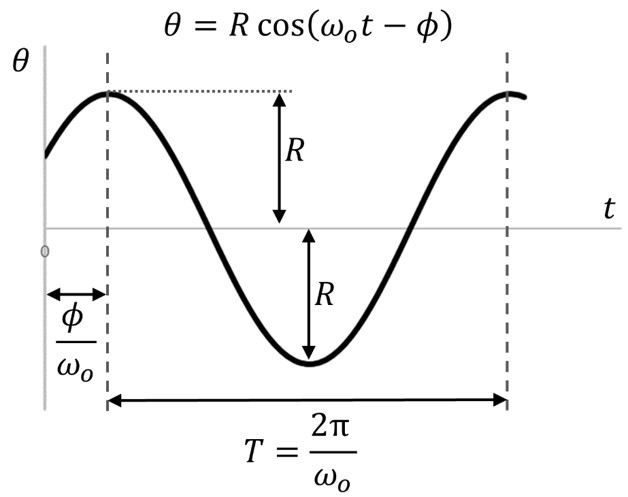
\includegraphics[height=1.5in]{graphofPendulum.jpg}
\end{image}

\subsection*{Preparing for and Conducting the Experiment}

\begin{problem}
Before proceeding, let’s consider the assumptions and simplifications behind this mathematical model.  Which of the following do you think is the most unrealistic assumption?
  \begin{multipleChoice}
      \choice[correct]{Neglecting any damping due to air resistance or other loss in motion.  }
      \choice{Using the small angle approximation $\sin\theta\approx\theta$ to greatly simplify the math.}
      \choice{Assuming that the gravitational constant g is in fact a constant.  }
      \choice{Neglecting the weight of the string and ignoring the size of the mass (treating it as a point). }
    \end{multipleChoice}
\end{problem}

Since we are expecting some damping, it will be good to record the experiment over several minutes, perhaps up to around five minutes.  Marks made on a nearby surface or a ruler or tape measure starting at the center position will help visualize the extent of the dampening as the oscillations decay in amplitude.  For small θ angles and sufficient lengths of string, the distance measured with these markings will be proportional to the angle.  Thus, it isn’t necessary to use a protractor  After our experiment, we will update the mathematical treatment to account for dampening.  For now, however, let’s estimate the period of the motion and see if it changes perceptibly over many cycles.  It may be best to conduct the experiment with another person to count oscillations, record data, or hold a video recording device.  It is recommended that only small angle oscillations be investigated.  Starting the object a distance of $20$ cm from the center position may be best for a string length of $1$ m.  You should simply release the object without imparting any initial velocity.  
The example in the following video provides a demonstration and a sample source of data.

%%%% insert videos 

\subsubsection*{Analysis of the Period}

A careful analysis of the video shows that $116$ oscillations occurred over four minutes ($240$ s).  We can estimate the average period by taking the total time in seconds and dividing by the total number of oscillations.  This average period is found to be about $2.07$ s, which is only slightly larger than our prediction of two seconds using the mathematical analysis above.  If we break the video down into segments, we find that this average period T does not increase or decrease in any noticeable way.  At first approximation, the period (and therefore the frequency) appears to be constant with time.  Using the formulas developed above, we could mathematically express our solution in either of the following two ways, the second being the amplitude phase form:

$$\theta\approx 11.3\cos (3.132t)+0.0104\sin (3.132t)\approx 11.3\cos(3.132t-0.00092)$$

\subsubsection*{Analysis of the Damping}

As anticipated, the amplitude of the oscillations does decay to about half its original value over the four minute time.  Note that $\tan\theta$ equals the linear distance divided by the length of the string.  Thus, going from an amplitude of $20$ cm to $10$ cm corresponds to a change in angle from $11.3^\circ$ to $5.7^\circ$.  Our mathematical model developed above misses damping completely.  The sines and cosines in the simple model will never decay.  Thus, while the period of oscillation seems constant, our model needs to be updated to include damping.

A new term incorporating the effect of damping, which is proportional to the angular speed of the pendulum, may be added to the previous differential equation

$$L\theta''+\alpha\theta'+g\theta=0$$

This is still a second order, linear, homogeneous problem.  As before, we can write it in standard form:
$$\theta''+\frac{\alpha}{L}\theta'+\frac{g}{L}\theta=0$$
Trench’s Theorem 5.2.1 provides a framework for understanding the solution.  A brief review of the mathematical treatment is included here.  This differential equation can be solved by proposing two individual solutions of the form $\theta=e^{rt}$.  This form is “plugged into” the differential equation, resulting in a characteristic equation $Lr^2+\alpha r+g=0$.  The quadratic equation can be used to find the characteristic values (roots) of r that satisfy the characteristic equation.  These two values of r are given by:
$$r=-\frac{\alpha}{2L}\pm i\frac{\sqrt{4Lg-\alpha^2}}{2L}$$
Where the imaginary number $i=\sqrt{-1}$ appears, because these roots are complex.

Note that in the undamped case explored above, $\alpha$ was zero, reducing to:
$r=\pm i\sqrt{g/L}=\pm i\omega_0$

In both cases, a generalized form of Euler’s formula may be used to deal practically with the imaginary component:
$$e^{a\pm qi}=e^{a}(\cos q\pm i\sin q)$$

The net result of all of these considerations is the solution to the differential equation with damping:

$$\theta=e^{\frac{-\alpha}{2L}t}\left[c_1\cos \left(\frac{\sqrt{4Lg-\alpha^2}}{2L}t\right)+c_2\sin\left(\frac{\sqrt{4Lg-\alpha^2}}{2L}t\right)\right]$$

There are still sine and cosine terms but there is also a decaying exponential that will limit the effective amplitude of oscillation, dampening it towards zero as time progresses.  Many oscillations occur, but each subsequent oscillation is slightly smaller than the one preceding it.  The decaying exponential term in the front defines the “envelope” of the solution: 

$$\theta=\pm\theta_0 e^{\frac{-\alpha}{2L}t}$$
We must find the value of α that would correspond to a halving of the amplitude (from $11.3^\circ$ to $5.7^\circ$) in $240$ s, as is depicted in the chart below: 
\begin{image}
 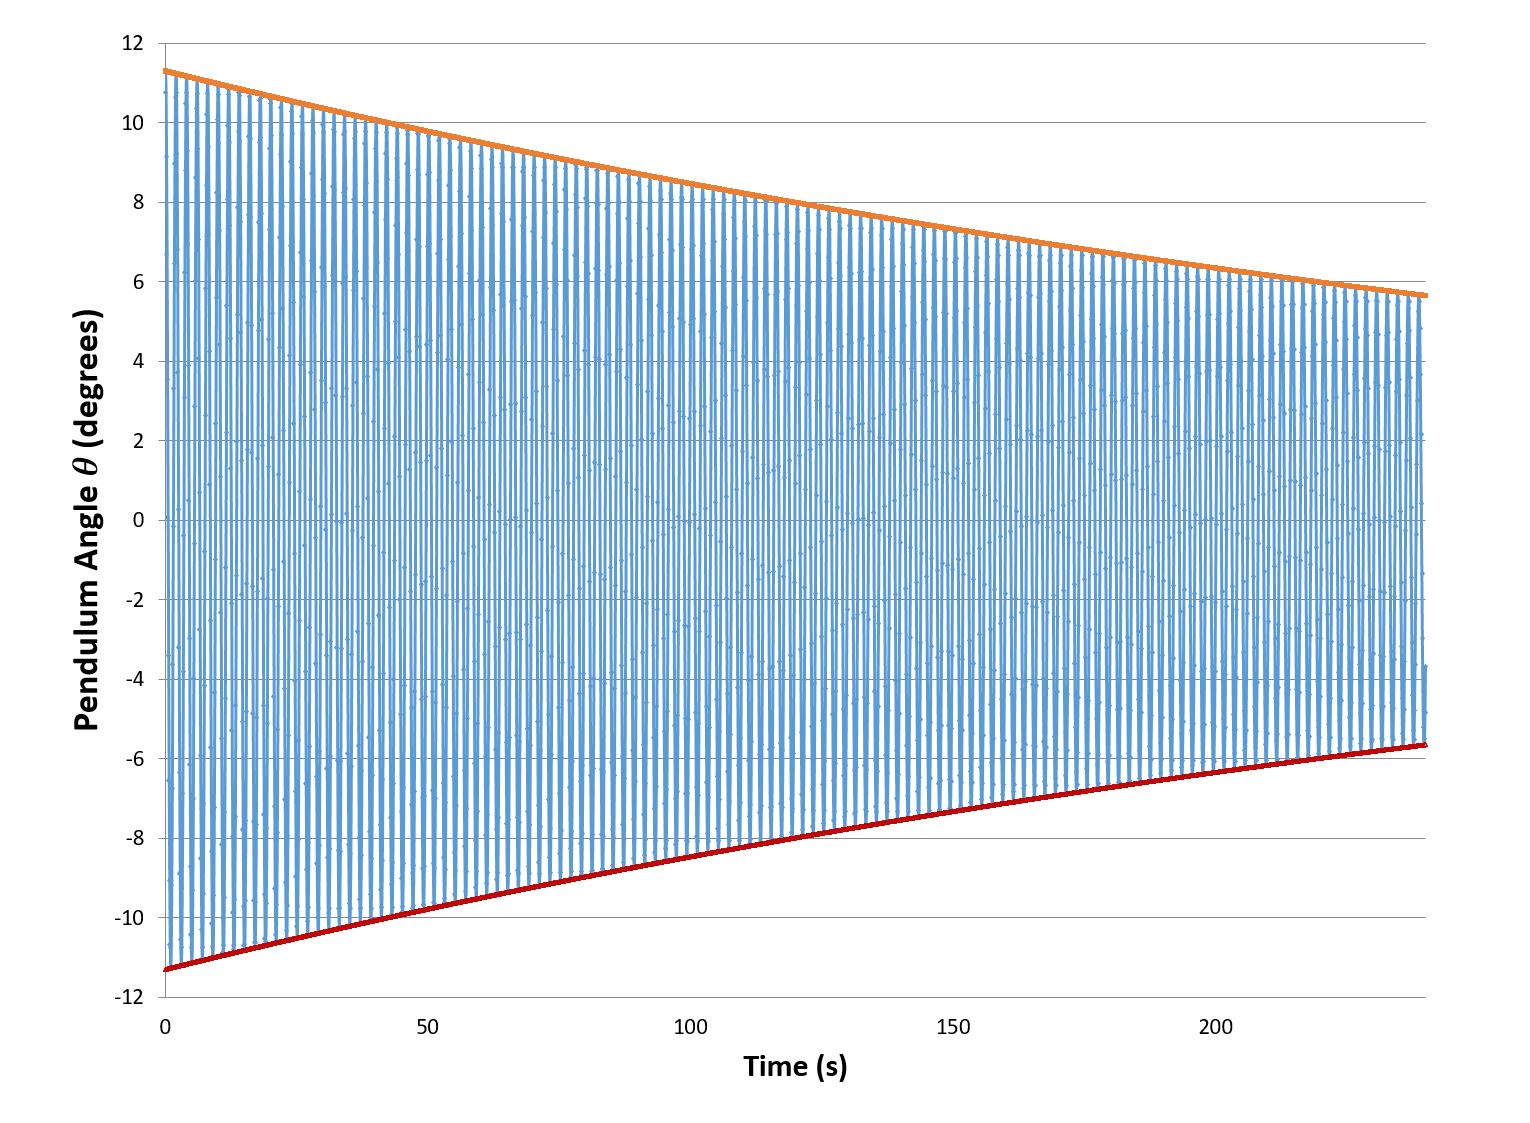
\includegraphics[height=1.5in]{simplePendulum.jpg}
\end{image}
In the beginning ($t=0$), the angle $\theta$ is the initial amplitude of oscillation $\theta_0=\sqrt{c_1^2+c_2^2}$.  We can calculate the value of $\alpha$ that corresponds to a certain amount of time leading to a fraction of initial amplitude:
$$\ln\left(\frac{\theta}{\theta_0}\right)=\left(\frac{-\alpha}{2L}\right)t$$
$$\alpha=\frac{2L}{-t}\ln\left(\frac{\theta}{\theta_0}\right)=\frac{2L}{t}\ln\left(\frac{\theta_0}{\theta}\right)$$

For the example shown in the video, $\frac{\theta}{\theta_0}=0.5$ when $t=240$ s.  thus, our estimate is that $\alpha\approx 0.00578$.  With initial conditions of $\theta (0)=11.3^\circ$ and $\theta'(0)=0$, we find the following solution approximately describing the motion in the example video:
$$\theta=e^{-0.0029t}\left[11.3\cos(3.132t)+0.0104\sin(3.132t)\right]$$
Note that the period and frequency of this motion are the same as in the undamped case.  This corresponds with the experiment and with our expectations from a purely mathematical perspective.  

\subsection*{Ideas for further experimentation}
Students may wish to try to identify other approximately simple pendula to model.  A small child in a swing slowing down may make for an interesting model, assuming that the child is unable to power their own swinging motion.  It is also worthwhile to try similarly sized objects of varying mass.  Since mass did not figure explicitly into the solution, students should be able to prove – by reviewing the math and confirming by experiment – that the magnitude of the mass does not directly impact the frequency or period of oscillation.  Another variation on this experiment would involve changing the length of the string and examining the effect on the outcome.
\end{document}
